
% this file is called up by thesis.tex
% content in this file will be fed into the main document

%: ----------------------- introduction file header -----------------------
% the code below specifies where the figures are stored
\graphicspath{{2/figures/}}

\chapter{Context}
\label{chp:context}

% Goals of this chapter
% ---------------------
% State of music informatics
% Reassessment of common practice
% Summary of findings
% Response to these findings: deep learning
%   Deep architectures
%   Feature learning

From its inception, many fundamental challenges in music informatics, and in particular those that focus on music audio signals, have received a considerable and sustained research effort from the community.
Referred to here as automatic music description, this area of study is based on the premise that if a human expert can experience or observe some musical event from an audio signal, it should be possible to make a machine respond similarly.
As the field of music informatics continues into its second decade, there are a growing number of resources that comprehensively review the state of the art in music signal processing across a variety of different application areas \cite{Klapuri2006Signal,Casey2008Content,Mueller2011Signal}, including melody extraction, chord estimation, beat tracking, tempo estimation, instrument identification, music similarity, genre classification, and mood prediction, to name only a handful of the most prominent topics.

% Things aren't solved; why?
After years of diligent effort however, many well-worn problems in content-based music informatics lack satisfactory solutions and remain unsolved.
Observing this larger research trajectory at a distance, it would seem progress is decelerating, if not altogether stalled.
For example, a review of recent MIREX\footnote{Music Information Retrieval Evaluation eXchange (MIREX): {http://www.music-ir.org/mirex/}} results motivates the conclusion quantitatively, as shown in Figure \ref{fig:mirex}.
The three most consistently evaluated tasks for more than the past half decade ---chord estimation, genre recognition, and mood prediction--- are each converging to performance plateaus below satisfactory levels.
Fitting an intentionally generous logarithmic model to the progress in chord estimation, for example, estimates that continued performance at this rate would eclipse 90\% in a little over a decade, and 95\% some twenty years after that; note that even this trajectory is quite unlikely, and for only this one specific problem (and dataset).
Attempts to extrapolate similar projections for the other two tasks are even less encouraging.
Furthermore, these ceilings are pervasive across many open problems in the discipline.
Though single-best accuracy over time is shown for these three specific tasks, a wider space of MIREX tasks exhibit similar, albeit more sparsely sampled, trends.

\begin{figure}
\begin{centering}
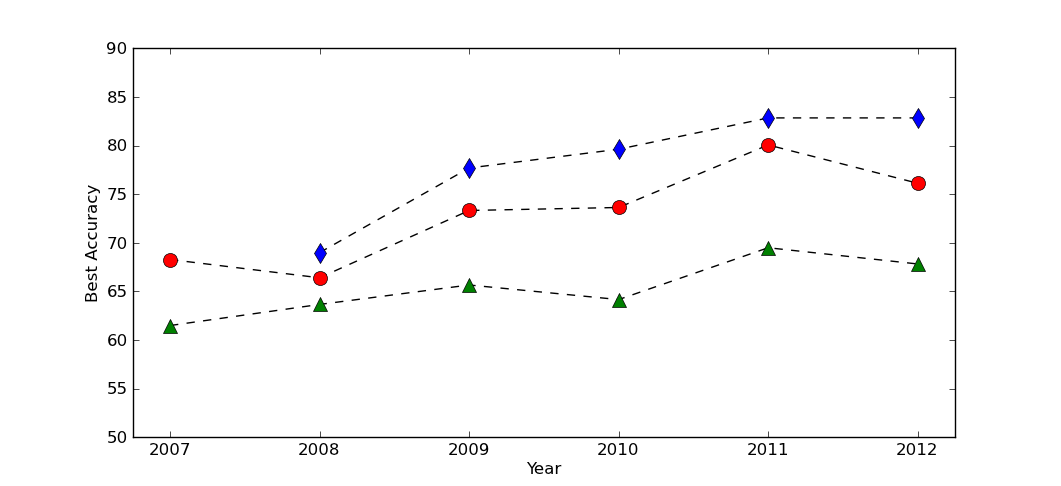
\includegraphics[width=\textwidth]{mirex2}
\caption{\emph{Losing Steam}: The best performing systems at MIREX since 2007 are plotted as a function of time for Chord Estimation (blue diamonds), Genre Recognition (red circles), and Mood Prediction (green triangles).}
\label{fig:mirex}
\end{centering}
\end{figure}

Recent research has additionally demonstrated that when state-of-the-art algorithms are used in more realistic conditions, i.e. larger datasets, performance degrades substantially \cite{BertinMahieux2012Largescale}.
Others have gone as far as to challenge the very notion that any progress has been made at all, due to issues of problem formulation and validity \cite{Sturm2014State}.
While the truth of the matter likely falls somewhere between ``erroneous results'' and ``sound science'', these varied observations encourage a critical reassessment of content-based music informatics.
Does content \emph{really} matter, especially when human-provided information has proven to be more useful than representations derived from the content itself \cite{Slaney2011Webscale}?
If so, what can be learned by analyzing recent approaches to content-based analysis \cite{Flexer2012MIREX}?
Do applications in content-based music informatics lack adequate formalization and rigorous validation \cite{Sturm2014Kiki}?
Is the community considering all possible approaches to solve these problems \cite{Humphrey2012Moving}?

Building on the premise that automatic music description is indeed valuable, this chapter is an attempt to answer the remainder of these questions.
Section \ref{sec:common} critically reviews conventional approaches to content-based analysis and identifies three major deficiencies of current systems: the sub-optimality of hand-designing features, the limitations of shallow architectures, and the short temporal scope of conventional signal processing.
Section \ref{sec:deep_learning} then introduces the ideas of deep architectures and feature learning in terms of music signal processing, two complementary approaches to system design that may alleviate these issues, and surveys the application of these methods in this domain.
Finally, Section \ref{sec:discussion} summarizes the concepts covered herein, and discusses why it is critical point in time for the music informatics community to consider alternative approaches.


\section{Reassessing Common Practice in Automatic Music Description}
\label{sec:common}

Despite a broad spectrum of application-specific problems, the vast majority of music signal processing systems adopt a common two-stage paradigm of feature extraction and semantic interpretation.
Leveraging substantial domain knowledge and a deep understanding of digital signal theory, researchers carefully architect signal processing systems to capture useful signal-level attributes, referred to as \emph{features}.
These signal features are then provided to a pattern recognition machine for the purposes of assigning semantic meaning to observations.
Crafting good features is a particularly challenging subproblem, and it is becoming standard practice amongst researchers to use precomputed features\footnote{Million Song Dataset} or off-the-shelf implementations\footnote{MIR Toolbox, Chroma Toolbox, MARSYAS, Echonest API}, focusing instead on increasingly more powerful pattern recognition machines to improve upon prior work.
While early research mainly employed simple classification strategies, such as nearest-neighbors or peak-picking, recent work makes extensive use of sophisticated and versatile techniques, e.g. Support Vector Machines \cite{Mandel2005Song}, Bayesian Networks \cite{Mauch2010Approximate}, Conditional Random Fields \cite{Sumi2012Music}, and Variable-Length Markov Models \cite{Chordia2011Predictive}.

\begin{figure}
\begin{centering}
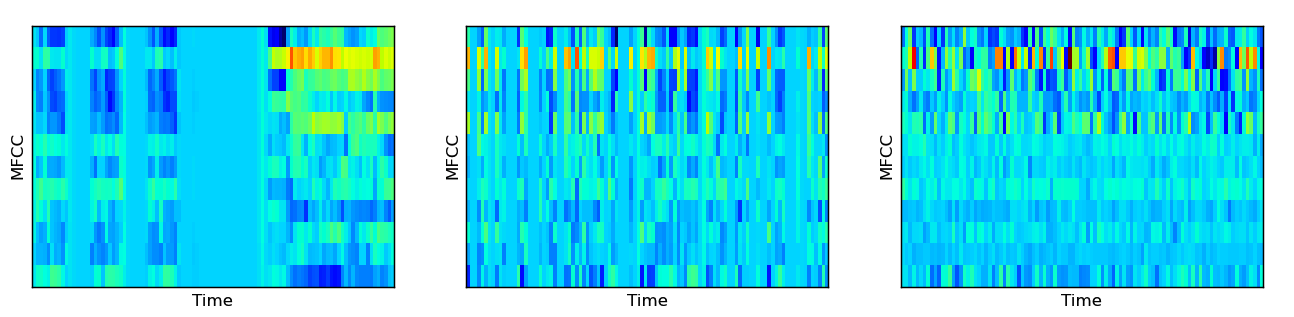
\includegraphics[width=\textwidth]{mtb_mfccs}
\caption{\emph{What story do your features tell?} Sequences of MFCCs are shown for a real music excerpt (left), a time-shuffled version of the same sequence (middle), and an arbitrarily generated sequence of the same shape (right). All three representations have equal mean and variance along the time axis, and could therefore be modeled by the exact same distribution.}
\label{fig:mfccs}
\end{centering}
\end{figure}

This trend of squeezing every bit of information from a stock feature representation is suspect because the two-tier perspective hinges on the premise that \emph{features are fundamental}.
Such representations must be realized in such a way that the degrees of freedom are informative for a particular task; features are said to be \emph{robust} when this is achieved, and \emph{noisy} when variance is misleading or uninformative.
The more robust a feature representation is, the simpler a pattern recognition machine needs to be, and vice versa.
It can be said that robust features \emph{generalize} by yielding accurate predictions of new data, while noisy features can lead to the opposite behavior, known as \emph{over-fitting} \cite{Bishop2006Pattern}.

The substantial emphasis traditionally placed on feature design demonstrates that the community tacitly agrees, but it is a point worth illustrating.
Consider the scenario presented in Figure \ref{fig:mfccs}.
Conceptually, the generic approach toward determining acoustic similarity between two music signals proceeds in three stages: short-time statistics are computed to characterize acoustic texture, e.g. Mel-Frequency Cepstral Coefficients (MFCCs); the likelihood that a feature sequence was drawn from one or more probability distributions is measured, e.g. a Gaussian Mixture Model (GMM); and finally, a distance is computed between these representations, e.g. KL-divergence, Earth mover's distance, etc. \cite{Berenzweig2004Large}.
Importantly, representing time-series features as a probability distribution discards temporal structure.
Therefore, the three feature sequences shown ---a real excerpt, a shuffled version of it, and a randomly generated one with the same statistics--- are identical in the eyes of such a model.
The audio that actually corresponds to these respective representations, however, will certainly not \emph{sound} similar to a human listener.

This bears a significant consequence: any ambiguity introduced or irrelevant variance left behind in the process of computing features must instead be resolved by the pattern recognition machine.
Previous research in chord estimation has explicitly shown that better features allow for simpler classifiers \cite{Cho2010Exploring}, and intuitively many have spent years steadily improving their respective feature extraction implementations \cite{Lyon2010Sound,Mueller2011Chroma}.
Moreover, there is ample evidence these various classification strategies work quite well on myriad problems and datasets \cite{Bishop2006Pattern}.
The logical conclusion to draw from this observation is that underperforming automatic music description systems are more likely the result of deficiencies in the feature representation than the classifier applied to it.

It is particularly prudent then, to examine the assumptions and design decisions incorporated into feature extraction systems.
In music signal processing, audio feature extraction typically consists of a recombination of a small set of operations, as depicted in Figure \ref{fig:simplearch}: splitting the signal into independent short-time segments, referred to as blocks or frames; applying an affine transformation, generally interpreted as either a projection or filterbank; applying a point-wise nonlinear function; and pooling across frequency or time.
These operations can be, and often are, repeated in the process.
For example, MFCCs are computed by filtering a signal segment at multiple frequencies on a Mel-scale (affine transform), taking the logarithm (a nonlinearity), and applying the Discrete Cosine Transform (another affine transformation).
Similarly, chroma features are produced by applying a constant-Q filterbank (affine transformation), taking the complex modulus of the coefficients (non-linearity), and summing across octaves (pooling).

\begin{figure}[t]
\begin{centering}
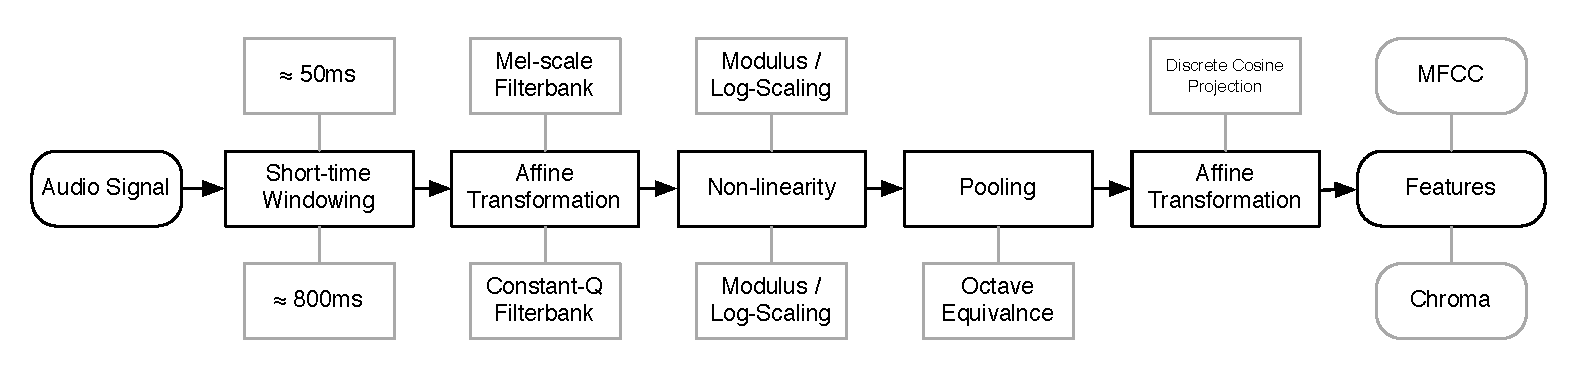
\includegraphics[width=\textwidth]{simplearch}
\caption{\emph{State of the art}: Standard approaches to feature extraction proceed as the cascaded combination of a few simpler operations; on closer inspection, the main difference between chroma and MFCCs is the parameters used.}
\label{fig:simplearch}
\end{centering}
\end{figure}


Considering this formulation, there are three specific reasons why this approach might be problematic.
First, though the data-driven training of classifiers and other pattern recognition machines has been standard for over a decade in music informatics, the parametrization of feature extractors ---e.g. choice of filters, non-linearities and pooling strategies, and the order in which they are applied--- remains, by and large, a manual process.
Both feature extraction and classifier training present the same basic problem: there exists a large space of possible signal processing systems and, somewhere in it, a configuration that optimizes an objective function over a dataset.
Though the music informatics community is privileged with a handful of talented researchers who are particularly adept at exploring this daunting space, crafting good features can be a time consuming and non-trivial task.
Additionally, carefully tuning features for one specific application offers no guarantees about relevance or versatility in another scenario.
As a result, features developed for one task are used in others for which they were not specifically designed.
The caveat of repurposing features designed for other applications is that, despite potentially encouraging results, they have yet to be optimized for this new use case.
Good features for chord estimation may blur out melodic contours, for example, and this information might be particularly useful for structural analysis.
In fact, recent research has demonstrated that better features than MFCCs exist for \emph{speech recognition} \cite{Mohamed2011Deep}, the very task for which they were designed, so it is reasonable to assume that there are better musical features as well.
The conclusions to draw from this are twofold: continuing to manually optimize a feature representation is not scalable to every problem, and the space of solutions considered may be unnecessarily constrained.


Second, these information processing architectures can be said to be \emph{shallow}, i.e. incorporating only a few non-linear transformations in their processing chain.
Sound is a complex phenomena, and shallow processing structures are placed under a great deal of pressure to accurately characterize the latent complexity of this data.
Feature extraction can thusly be conceptualized as a function that maps inputs to outputs with an order determined by its \emph{depth}; for a comprehensive discussion on the merits and mathematics of depth, we refer the curious reader to \cite{Bengio2009Learning}.
Consider the example in Figure \ref{fig:curvefit}, where the goal is to compute a low-dimensional feature vector (16 coefficients) that describes the log-magnitude spectrum of a windowed violin signal.
One possible solution to this problem is to use a \emph{channel vocoder} which, simply put, low-pass filters and decimates the spectrum, producing a piece-wise linear approximation of the envelope.
It is clear, however, that with only a few linear components we cannot accurately model the latent complexity of the data, obtaining instead a coarse approximation.
Alternatively, the \emph{cepstrum} method transforms the log-magnitude spectrum before low-pass filtering.
In this case, the increase in depth allows the same number of coefficients to more accurately represent the envelope.
Obviously, powerful pattern recognition machines can be used in an effort to compensate for the deficiencies of a feature representation.
However, shallow, low-order functions are fundamentally limited in the kinds of behavior they can characterize, and this is problematic when the complexity of the data greatly exceeds the complexity of the model.

\begin{figure}[t]
\begin{centering}
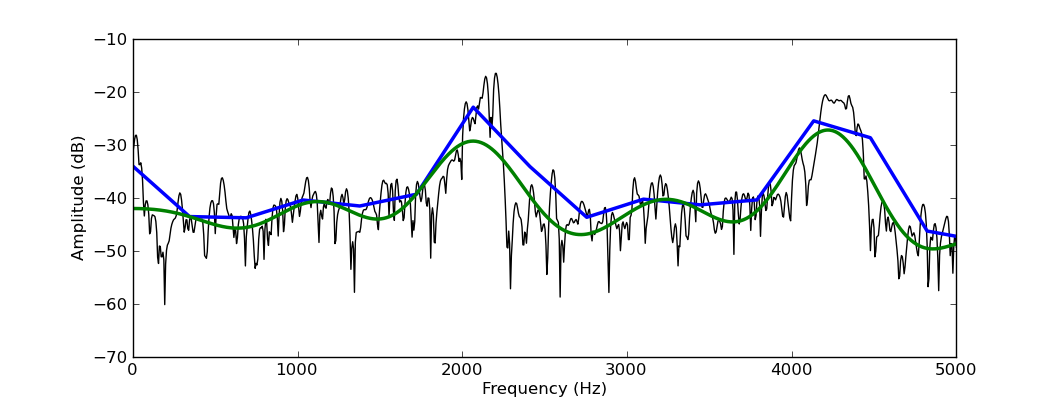
\includegraphics[height=1.5 in]{specfit}
\caption{\emph{Low-order approximations of highly non-linear data}: The log-magnitude spectra of a violin signal (black) is characterized by a channel vocoder (blue) and cepstrum coefficients (green). The latter, being a higher-order function, is able to more accurately describe the contour with the same number of coefficients.}
\label{fig:curvefit}
\end{centering}
\end{figure}

Third, short-time signal analysis is intuitively problematic because the vast majority of our musical experiences do not live in hundred millisecond intervals, but at least on the order of seconds or minutes.
Conventionally, features derived from short-time signals are limited to the information content contained within each segment.
As a result, if some musical event does not occur within the span of an observation ---a motif that does not fit within a single frame--- then it simply cannot be described by that feature vector alone.
This is clearly an obstacle to capturing high-level information that unfolds over longer durations, noting that time is extremely, if not fundamentally, important to how music is perceived.
Admittedly, it is not immediately obvious how to incorporate longer, or even multiple, time scales into a feature representation, with previous efforts often taking one of a few simple forms.
\emph{Shingling} is one such approach, where a consecutive series of features is concatenated into a single, high-dimensional vector \cite{Casey2008Analysis}.
In practice, shingling can be fragile to even slight translations that may arise from tempo or pitch modulations.
Alternatively, \emph{bag-of-frames (BoF)} models consider patches of features, fitting the observations to a probability distribution.
As addressed earlier with Figure \ref{fig:mfccs}, bagging features discards temporal structure, such that any permutation of the feature sequence yields the same distribution.
The most straightforward technique is to ignore longer time scales at the feature level altogether, relying on post-filtering \emph{after} classification to produce more musically plausible results.
For this to be effective though, the musical object of interest must live at the time-scale of the feature vector or it cannot truly be encoded.
Ultimately, none of these approaches are well suited to characterizing structure over musically meaningful time-scales.



\subsection{A Concise Summary of Current Obstacles}
\label{subsec:obstacles}
In an effort to understand why progress in content-based music informatics may be plateauing, the standard approach to music signal processing and feature design has been reviewed, deconstructing assumptions and motivations behind various decisions.
As a result, three potential areas of improvement are identified.
So that each may be addressed in turn, it is useful to succinctly restate the main points of this section:

\begin{itemize}

\item \textbf{Hand-crafted feature design is neither scalable nor sustainable}: Framing feature design as a search in a solution space, the goal is to discover the configuration that optimizes an objective function. Even conceding that some gifted researchers might be able to achieve this on their own, they are too few and the process too time-consuming to realistically solve every feature design challenge that will arise. \\
\item \textbf{Shallow processing architectures struggle to describe the latent complexity of real-world phenomena}: Feature extraction is similar in principle to compactly approximating functions. Real data, however, lives on a highly non-linear manifold and shallow, low-order functions have difficulty describing this information accurately. \\
\item \textbf{Short-time analysis cannot naturally capture higher level information}: Despite the importance of long-term structure in music, features are predominantly derived from short-time segments. These statistics cannot capture information beyond the scope of its observation, and common approaches to characterizing longer time scales are ill-suited to music.\\

\end{itemize}

\section{Deep Learning: A \emph{Slightly} Different Direction}
\label{sec:deep_learning}

Looking toward how the research community might begin to address these specific shortcomings in modern music signal processing, there is an important development currently underway in computer science.
\emph{Deep learning} is riding a wave of promise and excitement in multiple domains, toppling a variety of long-standing benchmarks \cite{Krizhevsky2012Imagenet,Hinton2012Deep}, while slowly permeating the public lexicon\cite{Brumfiel2014Deep,Markoff2012Scientists}.
Despite all the attention, however, this approach to solving machine perception problems has yet to gain significant traction in content-based music informatics.
Before attempting to formally define deep learning, though, it is useful to break down the ideas behind the very name itself and develop an intuition as to why this area is of particular interest.


\subsection{Deep Architectures}
\label{subsec:deep_architectures}

It was previously shown that deeper processing structures are better suited to characterize complex data.
Such systems can be difficult to design, however, as it can be challenging to decompose an abstract music intelligence task into a logical cascade of operations.
That said, the evolution of tempo estimation systems is a perfect example of a deep signal processing structure that developed naturally in the due course of research.

The high-level design intuition behind a tempo tracking system is relatively straightforward and, as evidenced by various approaches, widely agreed upon.
First, the occurrence of musical events, or onsets, are identified, and then the underlying periodicity is estimated.
The earliest efforts in tempo analysis tracked symbolic events \cite{Dannenberg1984Online}, but it was soon shown that a time-frequency representation of sound was useful in encoding rhythmic information \cite{Scheirer1998Tempo}.
This led to in-depth studies of onset detection \cite{Bello2005Tutorial}, based on the idea that ``good'' impulse-like signals, referred to as \emph{novelty functions}, would greatly simplify periodicity analysis.
Along the way, it was also discovered that applying non-linear compression to a novelty function produced noticeably better results \cite{Klapuri2006Analysis}.
Various periodicity tracking methods were simultaneously explored, including oscillators \cite{Large1994Resonance}, multiple agents \cite{Goto1995Realtime}, inter-onset interval histograms \cite{Dixon2007Evaluation}, and tuned filterbanks \cite{Grosche2011Extracting}.

\begin{figure}
\begin{centering}
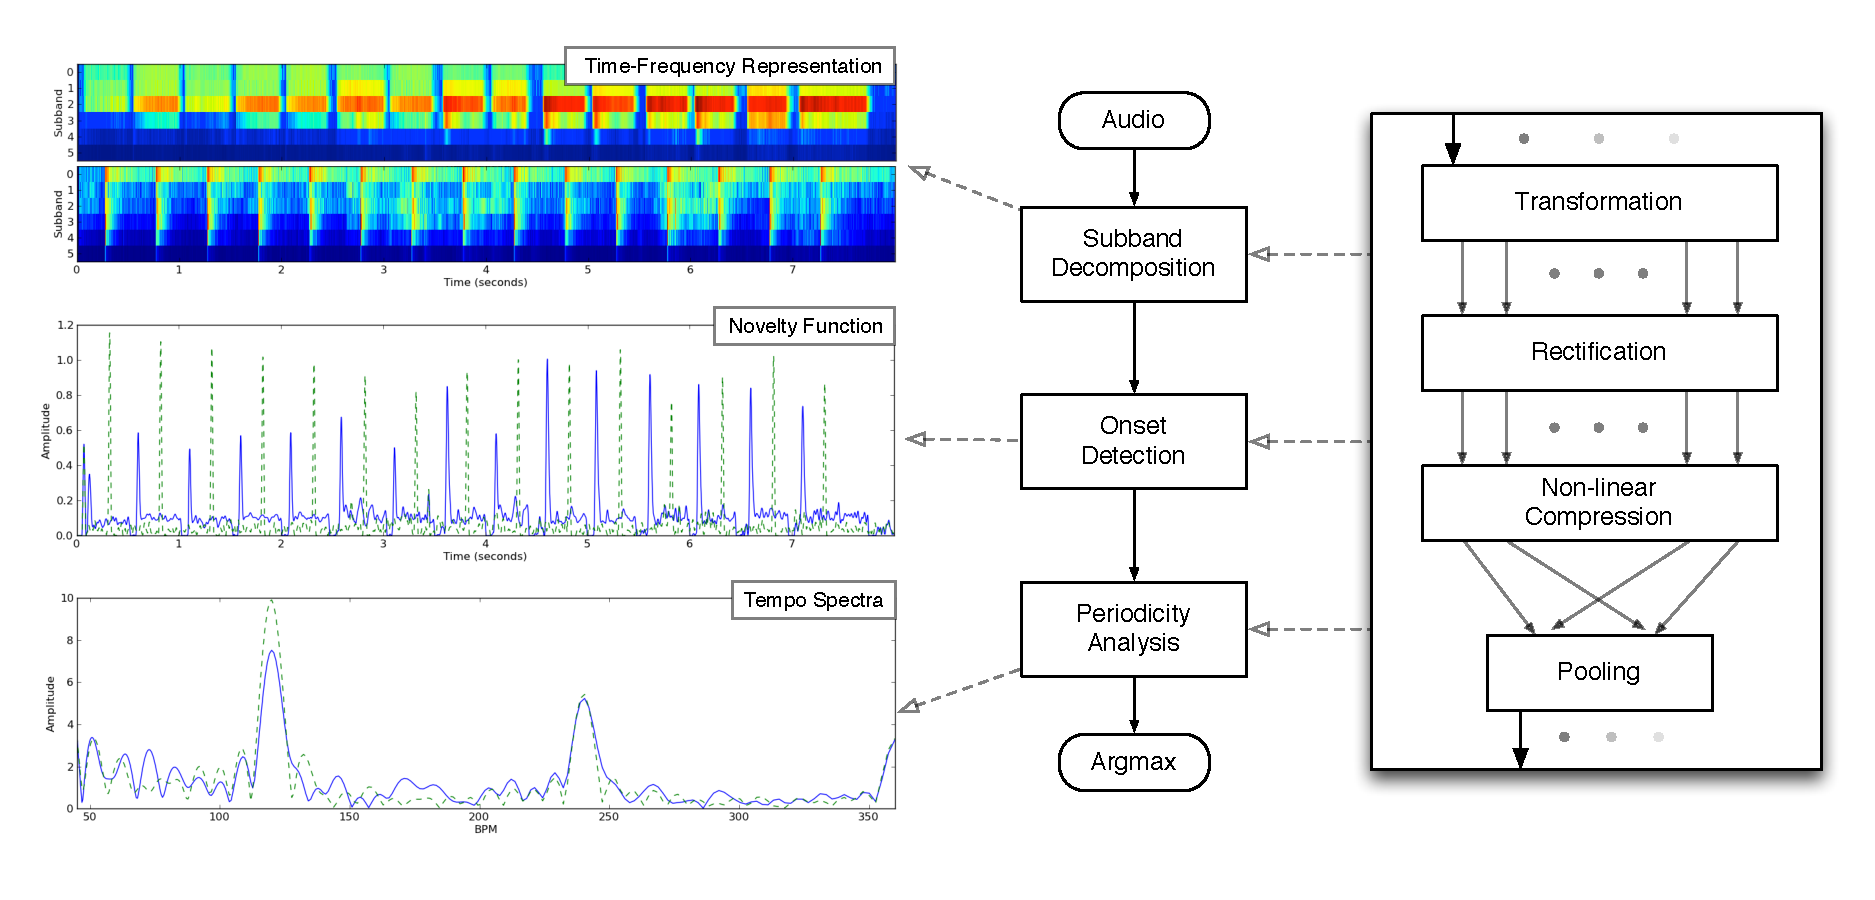
\includegraphics[width=\textwidth]{hierarchicaltecture}
\caption{\emph{A complex system of simple parts}: Tempo estimation has, over time, naturally converged to a deep architecture. Note how each processing layer absorbs a different type of variance ---pitch, absolute amplitude, and phase--- to transform two different signals into nearly identical representations.}
\label{fig:hierarchicaltecture}
\end{centering}
\end{figure}

Reflecting on this lineage, system design has, over time, converged to a deep learning architecture, minus the learning, where the same processing elements ---filtering and transforms, non-linearities, and pooling--- are replicated over multiple processing layers.
Interestingly, as shown in Figure \ref{fig:hierarchicaltecture}, visual inspection demonstrates why it is particularly well suited to the task of tempo estimation.
Consider two input waveforms with little in common but tempo; one, an ascending D Major scale played on a trumpet, and the other, a delayed series of bass drum hits.
It can be seen that, at each layer, a different kind of variance in the signal is removed.
The filterbank front-end absorbs rapid fluctuations in the time-domain signal, spectrally separating acoustic events.
This facilitates onset detection, which provides a pitch and timbre invariant estimate of events in the signal, reducing information along the frequency dimension.
Lastly, periodicity analysis eliminates shifts in the pulse train by discarding phase information.
At the output of the system, these two acoustically different inputs have been transformed into nearly identical representations.
Therefore, the most important lesson demonstrated by this example is how invariance can be achieved by distributing complexity over multiple processing layers.

As mentioned, not all tasks share the same capacity for intuition.
Multi-level wavelet filterbanks, referred to as scattering transforms, have also shown promise as a general deep architecture for audio classification by capturing information over not only longer, but also multiple, time-scales \cite{Anden2011Multiscale}.
Recognizing MFCCs as a first-order statistic, this second-order system yielded better classification results over the same observation length while also achieving convincing reconstruction of the original signals.
The authors demonstrate their approach to be a multi-layer generalization of MFCCs, and exhibit strong parallels to certain deep network architectures, although the parameterization here is not learned but defined.
Perhaps a more intriguing observation to draw from this work though is the influence a fresh perspective can have on designing deep architectures.
Rather than propagating all information upwards through the structure, the system keeps summary statistics at each timescale, demonstrating better performance in the applications considered.


\subsection{Feature Learning}
\label{subsec:feature_learning}

In traditional music informatics systems, features are tuned manually, leveraging human insight and intuition, and classifiers are tuned automatically, leveraging an objective criterion and numerical optimization.
For this reason, the quality of hand-crafted features is a crucial aspect of system design, as numerical optimization occurs downstream of manual feature design.
Many are well aware of the value inherent to good representations, and feature tuning has become a common, if tedious, component in music informatics research.
One such instance where this has occurred is in the tuning of chroma features.
Developed by Fujishima around the turn of the century \cite{Fujishima1999Realtime}, the last decade and a half has seen consistent iteration and improvement on the same basic concept; estimate the contribution of each pitch class over a short-time observation of audio.
Though initially devised for chord estimation, chroma features have been used in a variety of applications, such as structural segmentation \cite{Levy2007Comparison} or version identification \cite{Salamon2013Tonal}.

The fundamental goal in computing chroma features is to consolidate the energies of each pitch class according to a particular magnitude frequency representation.
One of the simplest ways to do so, given in Figure \ref{fig:all_weights}-(a), shows the averaging of pitch classes in a constant-Q filterbank, e.g. frequencies are spaced like the keys of a piano.
Later developments found that weighting the contributions of each frequency with a Gaussian window led to better performance, as shown in Figure \ref{fig:all_weights}-(b) \cite{Cho2014Improved}.
This improvement still took time to develop, further motivating the notion that other simple modifications remain undiscovered.
That said, this knowledge is attained by maximizing a known objective measure, such as classification accuracy in a chord estimation task.
Reflecting, this begs an obvious question: perhaps the parameters of a chroma estimation function could instead be \emph{learned} via numerical optimization?

\begin{figure}
\begin{centering}
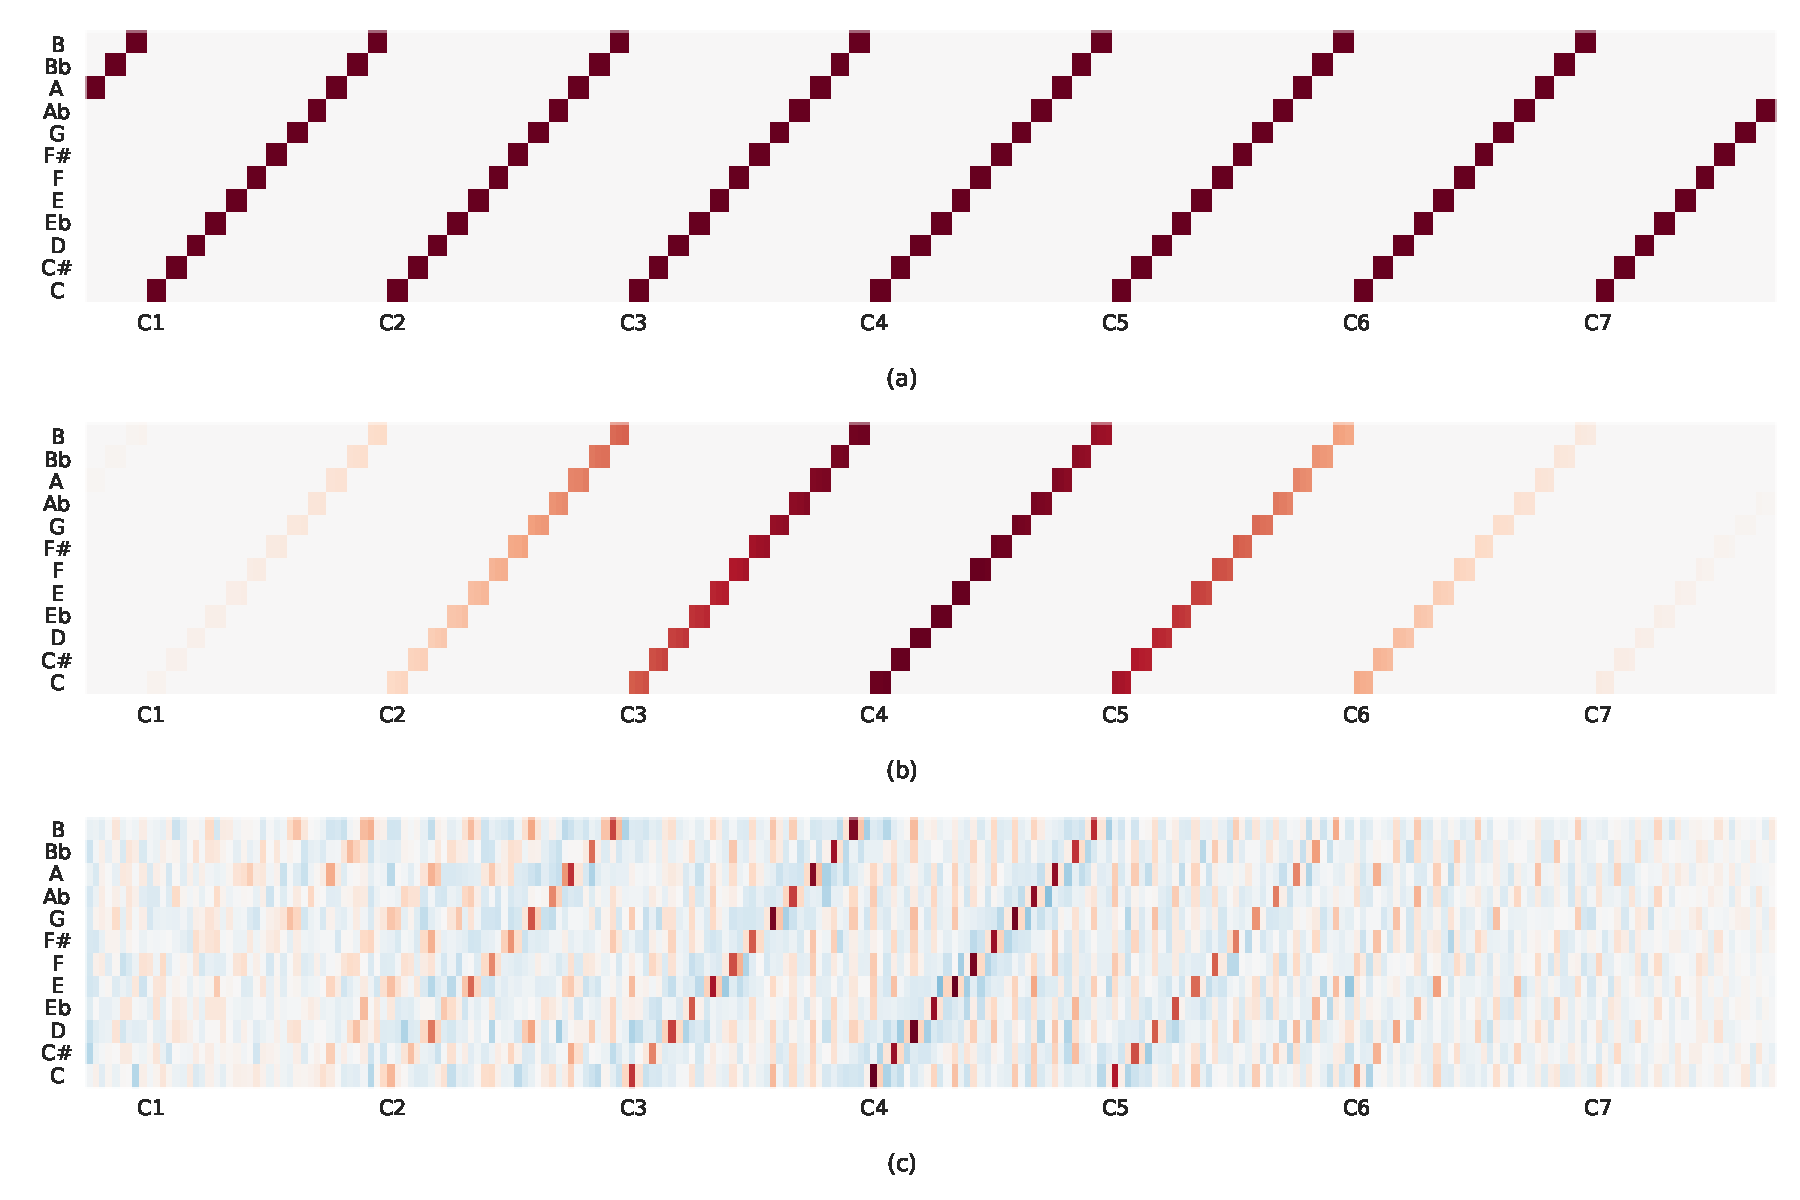
\includegraphics[width=\textwidth]{all_weights}
\caption{Various weight matrices for computing chroma features, corresponding to (a) uniform average, (b) Gaussian-weighted average, and (c) learned weights; red corresponds to positive values, blue to negative.}
\label{fig:all_weights}
\end{centering}
\end{figure}

Using the same general equation, a linear dot product between pitch spectra and a weight matrix, the mean-squared error is minimized between estimated chroma features and idealized ``target'' chroma features.
Reference chord transcriptions are used as an information source for the target chroma, producing binary templates from the chord labels.
The resulting weight matrix is illustrated in Figure \ref{fig:all_weights}-(c), and exhibits three significant behaviors.
First, the positive contributions to each pitch class are clearly seen at the octaves, as to be expected.
Second, the learned features corroborate the idea that the octave contributions should be weighted by a windowing function, and the one here looks vaguely Gaussian.
Third, and most importantly, the learned weights exhibit a small amount of suppression around each octave, shown in blue.
Similar to a Ricker wavelet \cite{Vaidyanathan1993Multirate}, negative sidebands serve to diminish wideband regions of energy, like those that found in percussion.


\begin{figure}
\begin{centering}
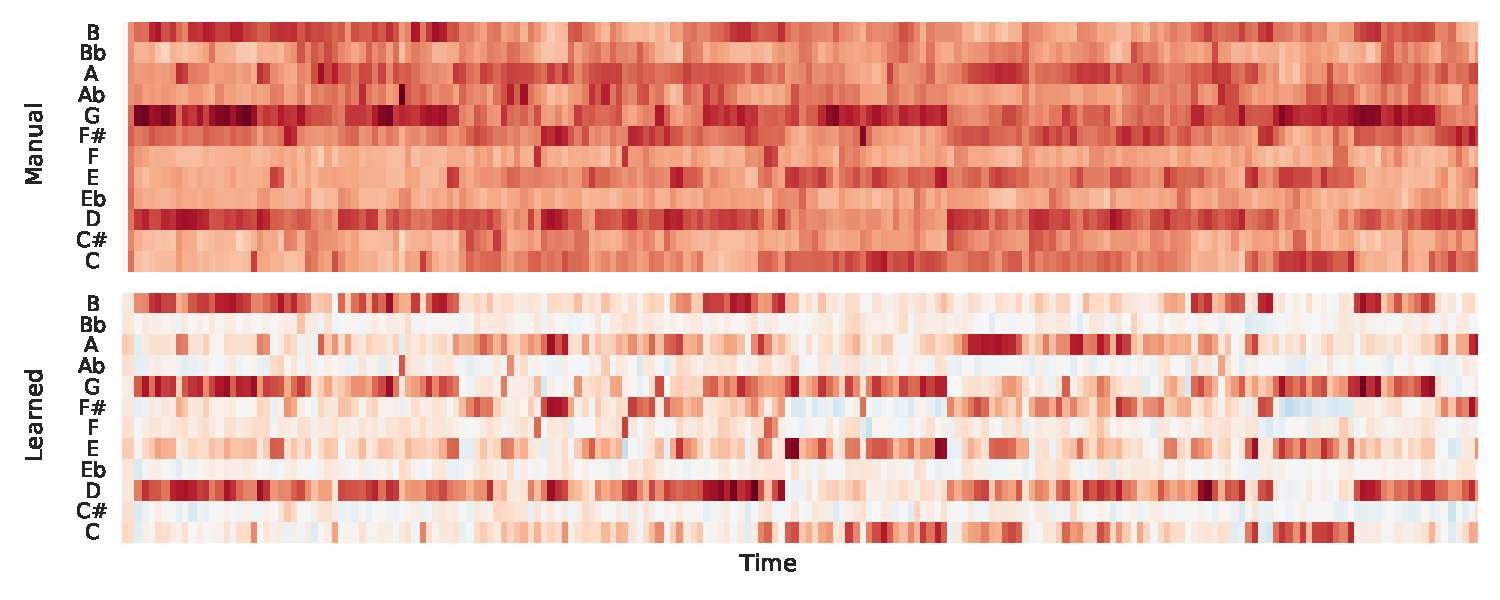
\includegraphics[width=\textwidth]{learned_chroma_TRAOIOP149E3AD2F51}
\caption{Comparison of manually designed (top) versus learned (bottom) chroma features.}
\label{fig:learned_chroma}
\end{centering}
\end{figure}

The chroma features obtained by these last two methods, (b) and (c), are shown in Figure \ref{fig:learned_chroma}.
The noise floor on the learned chroma features is much higher than the hand-crafted ones, as a direct result of the negative suppression in the learned weights.
While the idea of adjacent pitch energy suppression is novel, it is important to recognize a few things about this example.
Most importantly, it is curious to consider what other design aspects ``learning'' might help tease out from data.
The function considered here, a linear dot product, is very constrained, and ``better'' features are likely possible through more complex models.
Additionally, it is possible to directly inspect the learned weights because the system is straightforward; more complex models, however, will make this process far more difficult.


\subsection{Previous Deep Learning Efforts in Music Informatics}

While far from widespread, an increasing number of researchers have begun investigating deep learning to challenges in content-based music informatics.
% MLPs, DBNs
The most common form of deep learning explored for music applications focuses on such models to single frames of a music signal for genre recognition \cite{Hamel2009Automatic}, mood estimation \cite{Schmidt2011Modeling}, note transcription \cite{Nam2011Classification}, and artist recognition \cite{Dieleman2011Audio}.
% Convolutional networks
Meanwhile, the earliest instance of modern deep learning methods applied to music signals is found in the use of convolutional networks for the detection of onsets \cite{Lacoste2007Supervised}.
More recently, convolutional networks have also been explored for genre recognition \cite{Li2010Automatic}, instrument similarity \cite{Humphrey2010Nonlinear}, chord estimation \cite{Humphrey2011Learning, Humphrey2012Rethinking}, onset detection \cite{Schluter2014Improved}, and structural segmentation \cite{Ullrich2014Boundary}.
% Recursive models
Recursive neural networks, a powerful, if troublesome, model for sequential data, have also found success in chord transcription \cite{Boulanger2013Audio} and polyphonic pitch analysis \cite{Sigtia2014RNN}.
Additionally, predictive sparse decomposition (PSD) and other methods inspired by sparse coding have also seen a spike in interest \cite{Henaff2011Unsupervised, Nam2012Learning}, but while they make use of learning, neither of these systems are particularly deep.
Regardless, it is worthwhile to note that many, if not all, of these works have attained state of the art performance on their respective tasks, often in the first application of the method to the area.

% Symbolic?
% Beyond the space of audio signal processing, deep networks have also been used in to model symbolic music information.
% Conditional networks were demonstrated rhythm pattern analysis \cite{Battenberg2012}.
% Long short-term memory to model symbolic music sequences \cite{Eck2008}.
% Multiple viewpoint for similarity \cite{Cherla2014}


\section{Discussion}
\label{sec:discussion}

Recognizing slowing progress across various application areas in content-based music informatics, this chapter has attempted to develop an understanding as to why this might be the case.
Revisiting common approaches to the design of music signal processing systems revealed three possible shortcomings:
manual feature design cannot scale to every problem the field will need to solve;
many architectures are too shallow to adequately model the complexity of the data;
and there currently are not many good answers for handling longer time-scales.

In looking to other related disciplines, it seems deep learning may help address some, if not all, of these challenges.
Deep architectures are able to distribute complexity across multiple processing layers, thus being able to model more complex data.
Feature learning, on the other hand, allows for the automatic optimization of known objective functions, making it easier to discover signal-level characteristics relevant to a given task faster.
In fact, a handful of previous deep learning efforts within music informatics have already begun to demonstrate the promise of such methods.

Notably, these are crucial observations to make now for a variety of reasons.
From a practical standpoint, many in the research community are investing considerable effort in the curation of datasets.
While some, like \cite{Bittner2014Medleydb}, have gone to great lengths to clear licenses for the source audio signals, most use commercial recordings and thus sharing the original content is problematic.
As a result, it is becoming standard practice to apply a respected, but non-invertible, feature extraction algorithm over the original audio content and share the extracted statistics with the community, e.g. the Million Song Dataset \cite{Bertin2011Million}.
While these efforts are commendable, such datasets are ultimately limited by the feature extraction algorithm employed.
